\documentclass[a4paper,10pt]{article}
\usepackage[a4paper , top=38mm, right=38mm,left=38mm, bottom=38mm]{geometry}
\usepackage{hyperref}
\usepackage{xcolor}
\usepackage{subfiles} % subtex files package
\usepackage{graphicx} %figures and images
\graphicspath{{assets/images/}} % file path for images
\usepackage{blindtext} % for blind text
\usepackage{float}% float package
\usepackage{enumitem} % for enumerate & itemize
\usepackage{amsmath} % for math and equations
\usepackage{tabularx} % tables
\usepackage{adjustbox} %to adjust boxed content
\usepackage{tikz} % for tikz picture, graphs, etc
%\usepackage{pgfplots} % normal/logarithmic plots in two and three dimensions
%\usepgfplotslibrary{external} % pgfplots libraries
\usepackage[edges]{forest}  % for classification trees
\usetikzlibrary{shapes.geometric} % shapes tikz 
\usetikzlibrary{arrows.meta,arrows} % arrows for trees 
\usepackage{listings} %listings
\usepackage{xurl}
\usepackage{algorithm2e}
 \RestyleAlgo{ruled}
\usepackage{indentfirst}
\renewcommand{\abstractname}{\vspace{-\baselineskip}}

\setlength{\belowcaptionskip}{-10pt}

\DeclareSymbolFont{matha}{OML}{txmi}{m}{it}% txfonts
\DeclareMathSymbol{\varv}{\mathord}{matha}{118}

\usepackage{array}

\newenvironment{conditions}
  {\par\vspace{\abovedisplayskip}\noindent\begin{tabular}{>{$}l<{$} @{${}={}$} l}}
  {\end{tabular}\par\vspace{\belowdisplayskip}}
  

\hypersetup{
    pdftitle={Bitcoin (Blink) - Whitepaper},
    pdfauthor={Joby Reuben, Purva Chaudhari},
    pdfsubject={blockchain},
    pdfkeywords={blockchain, bitcoin, cryptocurrency,proofofspeed,projectblink,blink},
}

\font\myfontt=cmr12 at 10pt

\title{
 \large \textbf{Bitcoin (Blink) - Peer to Peer Global Cash System}\\
\vspace{6mm}
\scriptsize [WORKING-DRAFT-v0.1]
}
\author{ \myfontt Joby Reuben \\ \myfontt jobyreuben@gmail.com \and  \myfontt Purva Chaudhari \\ \myfontt purva@example.com}
\date{}
\begin{document}
\maketitle

\begin{abstract}
\noindent \textbf{Abstract :} Bitcoin's PoW is replaced with a propagation competition on blocks sent across validators under a certain time interval stamped with cryptographic proofs to claim fees and solve forks as per proof weight. To bring adaptable scalability the block sizes are decided on consensus among elected nodes of specific epochs to decrease waiting transactions. Gossip systems are replaced with a privacy-centered direct messaging system by constructing encrypted paths to deliver unconfirmed transactions \& confirmed blocks. Aside from bringing speed, we resolved the need for a single transaction fee token for a blockchain by bringing forth a novel non-custodial per-token staking system to offer users to pay in any token. Bitcoin as a currency will hold the security of the network, Layer-1 tokens with staking and yielding fees. Since Bitcoin script adapts a Turing-incomplete language and doesn't involve loops, the fees are imposed for renting UTXOs which makes transactions cheaper and the chain's ledger size optimized. We propose solutions for regulation revolving around taxation within the self-custody wallet ecosystem without compromising users' privacy. 

\end{abstract}

\section{Introduction}
Bitcoin Network and other altcoin blockchains with newer consensus and programmable money are unable to compete with centralized payment providers in speed and volume due to their sheer nature of inability to scale with centralization issues. Many consensus Models rely on external validation concepts, instead of rules tied to propagation itself. Imposing heavy reliance on users acquiring chain native tokens are adoption diminishing requirements that hide users from the wonders of blockchain technology for different regions of the world. Decentralized networks can effectively adapt to users' needs by 1. Increase Block Size 2. Decrease Block Time 3. Eliminate Low Efficient Nodes 4. Increase Node Joining Requirement. Retail Staking with non-custodial solutions encourages users to stake their Bitcoin to become a world reserve currency for every financial instrument with an additional restrictive monetary policy that helps to reduce volatility in times of recession.

Instead of storing UTXOs for an indefinite time which compromises storage, renting UTXOs and replacing them with a fingerprint after it expires without altering the block's Merkle root provides cheaper fees. With Bitcoin's unlocking script and use of sCrypt - a high-level language, developers can create custom scripts with - regulatory options involving various types of taxes within its UTXOs, offloading identity verification off-chain, with signatures instructing nodes to validate regulated payments with self-custody of tokens. Altcoins can be bridged one-way and collateralized for a stable coin directly used for staking and yielding fees along with Bitcoin bringing utility. Basic Banking solutions can be developed in Bitcoin Script whereas common computable programs can be deployed to Layer 2 EVM State Machine where nodes update the state by providing a Proof-of-Fee-Receipt paid in Bitcoin Layer. 
\section{Election}
Block size denotes the size of data that can be propagated across every producer node on the Bitcoin network, hence its success rate is directly dependent on the Bandwidth each node allocates for confirmed block transmission. Block size is not capped, but fixed every $n$ epoch which validates that every producer node on the network can send and receive the data size. Variable Block Size helps in scaling the network by increasing transactions per block if nodes upgrade and announce their bandwidth. A vote can be taken across producer nodes if there is an increase in unconfirmed transactions that cannot fit into a block. The network in consensus can forbid low bandwidth producer nodes from participating in the election, thus increasing the joining requirement and capacity to hold more transactions. 

As Bandwidth plays a major role in scalable infrastructure, nodes are required to have better of it to achieve maximum production rate per epoch, as elections will be conducted based on it and each node's honesty weight. Every Node willing to participate in the next epoch of block production, identity is given in its public keys published to the ledger onchain for definite calculations. For a random input value to commence the election, from a range of blocks of an epoch ($n-m$) confirmed Blocks Merkle Chain Root which is constructed by validators is taken. For a $2^{256}$ possible outcome, $n$ times it is divided evenly and finds if any block's MCR lies on the selected $r$ range. With the MCR input, blocks are randomly assigned to each epoch producer without consecutive assignments. 

\section{Staking}
Bitcoins can be staked for public keys with specified token IDs where the collateral can be used only once for a block. This results in a stake per token per block employing the throughput (tps) per token basis. Each token per block collateral requirement ($y$) is given in market price (USD) by taking the median volume of all the blocks of the previous epoch. Staked Bitcoins can be withdrawn anytime, without a vesting period except at the time of producing the block. This brings a retail and non-custodial solution as opposed to security deposit-type PoS chains. As slashing is done directly to fees, delegators won't lose their stakes. Bitcoins can be staked to a specific node that chooses to include the stake by collateralizing or locking in its allocated block. In this way, for a specific token's transaction to be included in a block, the first of transactions should prove the collateral. During staking, an additional interest rate ($r$) is added to restrict the free flow of tokens to increase demand in exchanges by imposing a timelock of 500 epochs. This interest rate is decided by analyzing the market price of current and previous epochs.

\begin{equation}
x=\epsilon_{n-2}[\widetilde{x}( \{b_1, b_2, \dots b_n\} (\sum_0^n \Psi T_h(b_n)))]
\end{equation}
\begin{equation}
\forall r (T_h(\epsilon_n)) =  r(T_h(\epsilon_{n-1}))  +  (\frac{C_{\epsilon_{n-3}} - C_{\epsilon_{n-2}}}{10  \cdot  C_{\epsilon_{n-2}}}) \geq 10^{-2}
\end{equation}
\begin{equation}
y=x+ [r (T_h(\epsilon_n)) \cdot (x)]
\end{equation}
where:
\begin{conditions}
\widetilde{x} & Median Value\\
T_h & Token ID Hash\\
\epsilon_n & Current Epoch\\
\epsilon_{n-k} & Target Epoch\\
b_n & Target Block\\
\Psi & UTXO outs in Market Price\\
r & Interest Rate\\
C & Closing Market Price $(\epsilon_n)$\\
y & $x+r$ for a $T_h(\epsilon_{n}(b))$
\end{conditions}

Additionally, a new collateralized floating-rate coin can be issued from lending altcoins which can be used for staking to receive yield benefits.
\section{Regulation}
Regulating cryptocurrencies via centralized exchanges \& custodians risks funds and doesn't encourage a self-custodial ecosystem. A regulator must have the authority to sign/approve transactions. Whitelisting specific hashed addresses belonging to specific countries verified and signed by Government assigned Client Wallets or Regulators by either doing full KYC or minimal such as Mobile Number based OTP verification could work with maximum privacy.

 UTXOs are stamped with region proof on their unlocking script based on specific spending conditions that will only allow a transaction onchain if taxes are deducted properly. Bitcoin scripts can work efficiently and securely as opposed to Turing complete smart contracts in this case. Tax models such as Capital Gains Slabs can be issued by governments independently and trustlessly and are validated in script execution. External taxes such as TDS, Sales tax can be imposed off-chain as it's flexible to do so.
\section{Messaging}
\begin{figure}[H]
\begin{center}
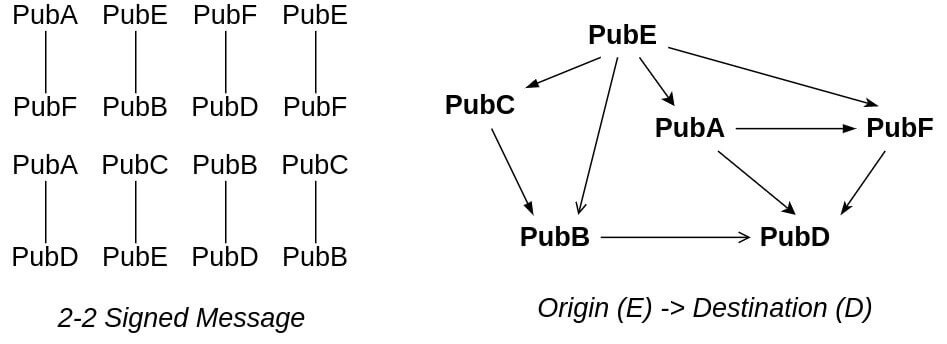
\includegraphics[width=8cm]{topology}
\caption{Topology}
\end{center}
\end{figure}
Delivery of unconfirmed transactions to nodes play important role in finality. Shared Mempools collude the network with duplicated data that results in a poor choice of transactions to include in a block. Miners take only transactions with higher fees. A direct-messaging system should be deployed with messaging instructions specific to each party as opposed to a gossip network. Paths are attached with unconfirmed transactions directly from the constructed network graph available to all nodes with public keys as identities. Two peered parties mutually sign a 2-2 random message for every $x$ block, and are gossiped across the network to identify the connection as online. From all the signed random messages proving each pubkey signature can display a network topology map from the point of reference node. 
Paths have encrypted instructions and a secret number associated with each party's public key that can be proved to increase the production rate in the next epoch. Nodes route the transaction between the origin and the destination where producers can attach the transaction to their allocated block. 
Since the stake information is available publicly client wallets constructing the transaction with path shall assume and select possible blocks that will add the transaction to it at the earliest. Nodes only receive the transactions which they need to include and client wallets should construct shorter paths to provide the best user experience.
\section{Propagation}
\begin{figure}[H]
\begin{center}
\includegraphics[width=11cm]{Snips}
\caption{Snips}
\end{center}
\end{figure}
A Block is collectively validated but constructed as snips - divisible block chunks by the producer and directly messaged to most of the current epoch's producer nodes with routing instructions to gossip across the network. Each snip references the previous snip's hash similar to the chain of blocks for proper identification of each block's snips. For a block of an epoch, a competition to deliver all snips under $x$ time intervals is required to win rewards and avoid slashing of fees. When a block fails to win shall be minted until its last snip which may contain rewards. VDF proofs are attached for every snip during routing to declare the state of each block's competition after resolving forks based on proofs weights. Failed block fees are slashed by sending them to a burn address by the next block height producer. Each failed block with various categories shall result in decreased block production for the node in the next epoch indirectly slashing bandwidth costing capital which instructs nodes to act honestly with the performance required for the epoch. Null-Blocks are minted by $n-1$ block producer with the VDF proofs. Some of these negative weights are temporary and permanent and some weights are incentive as it increases its maximum achievable block production in the next epochs. 

To synchronize time, each node's hash rate per second of a specific hash function is proved cryptographically onchain and taken in multiples of a common hardware's hash rate. This Individual hash-rate proof is also provided along with bandwidth proof for every epoch which trustlessly synchronizes all nodes as a single hardware producing continuous hashes concated with all snips providing cryptographic timestamped proofs to announce each epoch's block time under which all snips have to arrive and win the time-based propagation competition. The competition is termed Proof of Speed.

\section{Rewards}
Rewards are given for each snip hash as block time varies in this implementation to provide faster finality of transactions. Since a year's total newly minted bitcoins are definite and the common hardware's hash rate per year is also definite and used to synchronize various nodes' hash rates, new bitcoins can be supplied for each allocated block. From the origin snip hash to the final snip of a block, the total index of hashes is taken to validate the total bitcoins the block can issue. While Tax outputs are attached as zero input transactions within the snip it contains, the fee outputs when accounted mark the end of the block. 

During staking producers announce their accepted tokens for which they will directly withdraw the commission. For other tokens, delegators can stake with a condition that their stake in bitcoins or the accepted stake token will be traded for the collected fees. During the commission withdrawal of non-accepted tokens, the producer will deposit collected fees to delegators and inflate the stake to LP token 1:1 ratio to withdraw the collateral. Users can pay in any token, delegators incur the risk, and producers get paid to validate transactions.

\section{Renting}
Instead of taking the Merkle roots of all the transactions inside a block, a snip's Merkle root is taken and linearly hashed to find the Merkle Chain root. \\


\begin{figure}[h]
\begin{center}
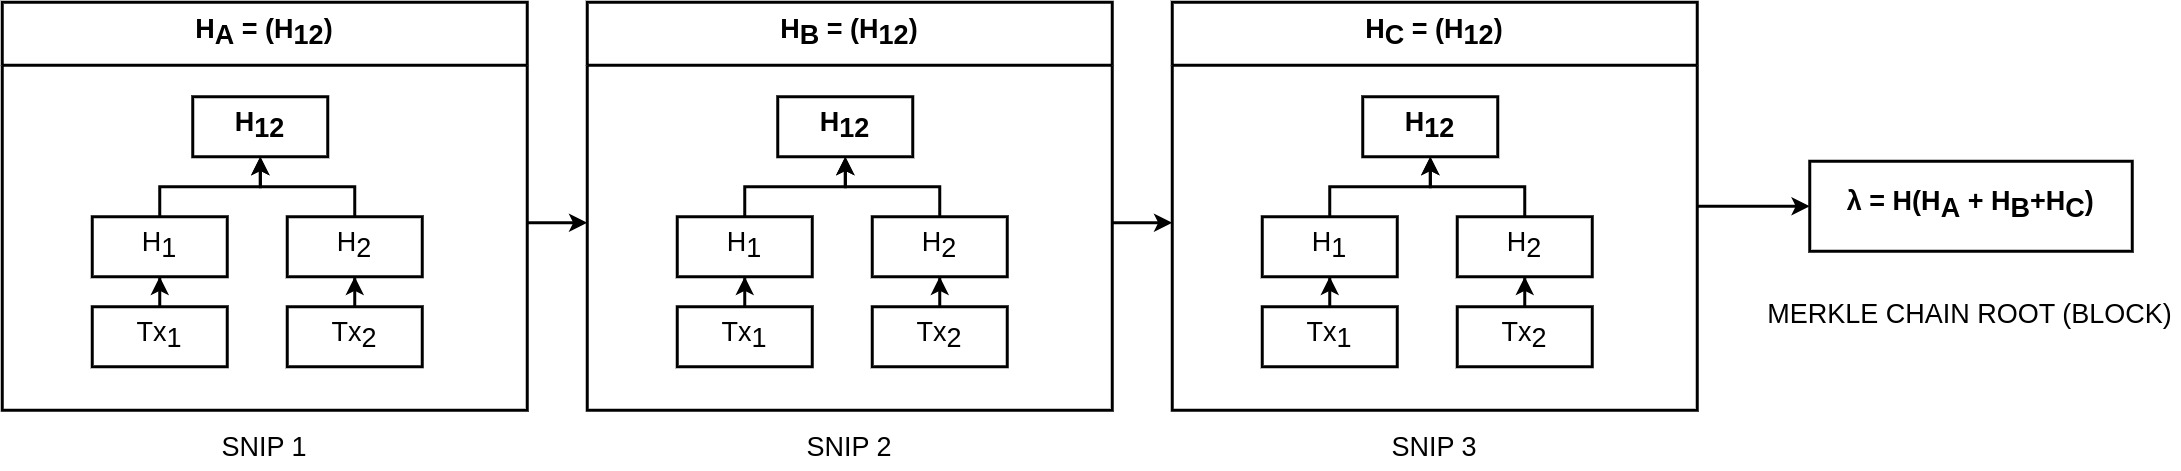
\includegraphics[width=13cm]{merklechain}
\caption{Merkle Chain}
\end{center}
\end{figure}

\indent Since snips can be rejected by validators, it is unsure to predict a Merkle chain root giving it a purely randomized value. Inside a snip contains parsed transactions whose hashes are taken to find the snip's Merkle root can be pruned if the UTXOs are spent, burnt, or expired. Each UTXO expiry block height is embedded in its script, and can be scanned by nodes, and pruned to optimize their data storage. Client Wallets can store each of their users' transaction history and can be audited onchain using Merkle chain roots. Renting rates can be given in market price independently voted by producer nodes for every epoch per byte per block. Users cannot directly pay for rent, but rather each new UTXO created is charged a transfer fee in the range of 0.05\% - 0.005\% decided based on the total volume of all transactions settled on previous epochs.
\begin{equation}
5 \cdot 10^{-4} \leq \Delta f \leq 5 \cdot 10^{-5} == \sigma [\Psi (\epsilon_{n-3}, \epsilon_{n-2})] > 0.75
\end{equation}
\begin{equation}
f'=f+x \begin{cases}
x=+5 \cdot 10^{-6}, & \text{if } \Psi (\epsilon_{n-3} > \epsilon_{n-2})\\
x=-5 \cdot 10^{-6}, & \text{otherwise}
\end{cases}
\end{equation}
where:
\begin{conditions}
F & UTXO value $\times f'$ 
\end{conditions}

 Transfer fee charges more fees for higher value utxos and less for lesser value utxos bringing ease of transacting for retailers. According to how much each utxo pays for a transfer fee, an expiry date is set. UTXOs doing state updates will not be charged and can combine UTXOs to a single balance holding UTXO with increased expiry value. This encourages users to store a single UTXO per wallet reducing transaction fees and also incentivizes nodes, clients, etc.  
 
\section{Forks}

\begin{figure}[H]
\begin{center}
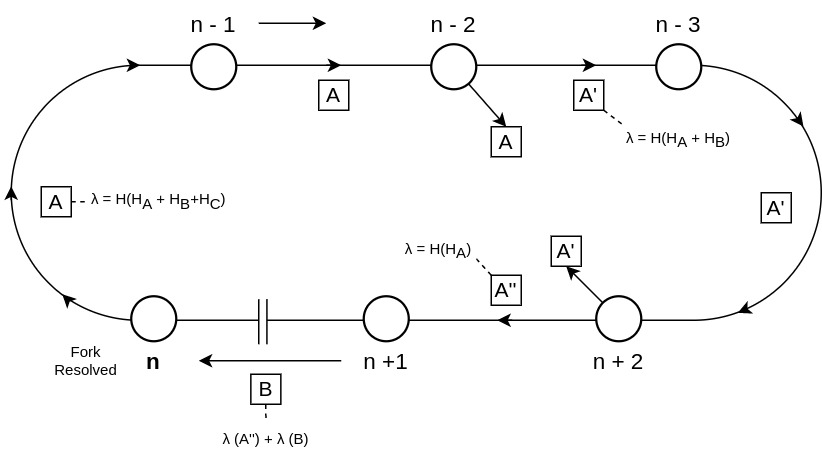
\includegraphics[width=10cm]{fork}
\caption{Resolving Forks}
\end{center}
\end{figure}


Confirmed blocks as snips are streamed with an included path that propagates across every producer in a backward ring manner. The snips are attached with VDF proofs by producers which provide proof of block time. Forks arise when different producers reject extra snips, this can be resolved by the very next block, providing instant finality to users. Additionally, negative weights are added if the fork arises after the first destination node of the path with VDF evaluation. Bandwidth upgrades are needed for the nodes which initiate the fork and directly instruct the origin block size should be decreased.
\begin{align}
\lambda (B_A) = H(H_A+H_B+H_C) \\
\lambda (B_{A'}) = H(H_A+H_B)\\
\lambda (B_{A''}) = H(H_A)  \\
\lambda (B_{B}) = H(\lambda(B_{A^?}) + \lambda(B_{B^?}))
\end{align}
For a block, possible Merkle Chain Roots are constructed and forks are resolved. The next blocks will have the input hash value of the previous block's Merkle Chain Root. To avoid influence by the first destination node, path planning can be randomized but must include the next block producer as the final destination.
\section{Oracles}

\section{Tokens}
Tokens can be created and deployed natively to UTXOs. Bridging assets from one chain to bitcoin would be more secure one-way since the chain involves taxations passively until the time of spending. Smart contracts can be deployed in other chains to provide a one-time signature associated with a private key which can be proved onchain and mint new tokens with token ids mapped to each UTXO. Tokens in Bitcoin can inherit the security of the network and also offer to pay fees for the same tokens as well. Key decentralized, non-security tokens will be selected. 
 
\section{Maintenance}
For the sustainability of the project and active development, the developers of project blink can set up a DAO for decisions involving protocol changes and soft forks to register government tax wallets. Developers can be actively rewarded by the DAO restricting a minimal commission on producer fees. Only the accepted tokens and staked tokens are sent to the DAO treasury. Since there are no parameter upgrades on the current implementation, decisions are solely focussed on building additional modules for maximal user adoption financed from DAO treasury instead of donations.

\section{Future}

Collateral coin, Exchanges, Lending \& Borrowing, Insurance, Mirrored Wallets, Obscuring Amounts, Ring Signatures decryption by government, Layer 2 Cash System, EVM Layer with unique Proof of Fee receipt consensus model, removing EOAs, Balances, Purely for Logic, and State update. NFTs,\\
\begin{center}
\nocite{nakamoto2008bitcoin}, \nocite{poon2016bitcoin} , \nocite{yakovenko2018solana}, \nocite{wood2014ethereum}, \nocite{rai2020}, \nocite{Stateful}
\end{center}


\bibliographystyle{ieeetr}
\bibliography{citation.bib}
\appendix
\noindent \Large \textbf{Appendix}
\normalsize
\section{Zk Circuits}
@Purva
\subsection{Bandwidth Proof}
\subsection{VoC Vote}
\subsection{Hashrate Proof}
\section{Election}
@Joby VoC till announcement
\section{Regulated Wallets}
@Joby Tree of Accepted Wallets - nonchangeable
\section{Tax Scripts}
@Ajay Pseudocode
\begin{algorithm}
\caption{Pay to Regulated Key Hash}
Here
\end{algorithm}
\section{Stake Script}
@Ajay Pseudocode
\begin{algorithm}
\caption{Staking}
Here
\end{algorithm}
\section{Routing Path}
\section{Routing Reward}
\section{Time Proof}
@Joby - VDFs included in snips
\section{21 Million}
@Ajay - Pseudocode
\begin{algorithm}
\caption{Yearly Allocation}
Here
\end{algorithm}
\section{Fee Withdrawal}
@Ajay - Pseudocode
\begin{algorithm}
\caption{Fee Withdrawal}
Here
\end{algorithm}

\section{Oracle Scripts}
@Ajay - Pseudocode
\begin{algorithm}
\caption{Oracle Scripts}
Here
\end{algorithm}


\end{document}